\section{Algebraic Diagrammatic Construction}
With the basic knowledge of second quantization, perturbation theory and Green function, we can then start discussing ADC.
We know that we can calculate ionization potentials, electron affinities and ground state energy from Green function by \ref{spectralrepresentation} and \ref{greenenergy}.
We also know that we can use Wick's theorem and Feynman rules for Abrikosov diagram to calculate each order of Green function.
Thus, as least in principle, we can practically calculate some physical quantities.
However, a finite perturbation expansion, e.g., through third order, e.g.
\begin{equation}
\boldsymbol{G}(\omega)=\boldsymbol{G}^{0}(\omega)+\boldsymbol{G}^{(2)}(\omega)+\boldsymbol{G}^{(3)}(\omega)+O(4)
\end{equation}
does not result in a useful approximation scheme to determine the physical quantities of interest.
The reason is that the components $G_{pq}(ω)$ are analytical functions, and a finite perturbation expansion does not recover the proper analytical structure.
What is needed here is to sum the perturbation expansion, even if only partially, through infinite order.
We will introduce two ways, which are Dyson approach and Non-dyson approach to such infinite summation.

\subsection{Dyson Approach}
The Green function can be written as:

\begin{minipage}{0.08\textwidth}
	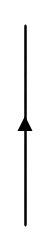
\includegraphics[height=3cm]{./figures/free.png}
\end{minipage}
\begin{minipage}{0.05\textwidth}
	+
\end{minipage}
\begin{minipage}{0.08\textwidth}
	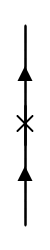
\includegraphics[height=3cm]{./figures/diagramA.png}
\end{minipage}
\begin{minipage}{0.05\textwidth}
	+
\end{minipage}
\begin{minipage}{0.12\textwidth}
	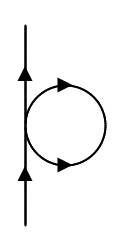
\includegraphics[height=3cm]{./figures/diagramC.png}
\end{minipage}
\begin{minipage}{0.05\textwidth}
	+
\end{minipage}
\begin{minipage}{0.1\textwidth}
	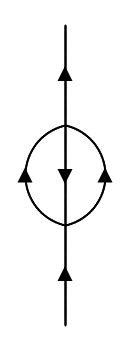
\includegraphics[height=3cm]{./figures/order2.png}
\end{minipage}
\begin{minipage}{0.2\textwidth}
	+ \qquad \dots
\end{minipage}

We can see that except the first one, all of the diagrams both start and end with a free Green function line.
Thus, we can define improper self-energy part $\widetilde{\Sigma}_{p q}\left(t_{1}, t_{1}^{\prime}\right)$ as the infinite summation of the parts between two free Green function lines in each diagram:

\hspace{0.4\textwidth}
\begin{minipage}{0.08\textwidth}
	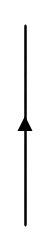
\includegraphics[height=3cm]{./figures/free.png}
\end{minipage}
\begin{minipage}{0.05\textwidth}
	+
\end{minipage}
\begin{minipage}{0.05\textwidth}
	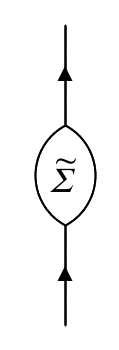
\includegraphics[height=3cm]{./figures/newdyson.png}
\end{minipage}

Algebraicly, it reads:
\begin{equation}
	G_{p q}\left(t, t^{\prime}\right)=\delta_{p q} G_{p}^{0}\left(t, t^{\prime}\right)+\int \mathrm{d} t_{1} \int \mathrm{d} t_{1}^{\prime} G_{p}^{0}\left(t, t_{1}\right) \widetilde{\Sigma}_{p q}\left(t_{1}, t_{1}^{\prime}\right) G_{q}^{0}\left(t_{1}^{\prime}, t^{\prime}\right)
\end{equation}
or
\begin{equation}
	G_{p q}(\omega)=\delta_{p q} G_{p}^{0}(\omega)+G_{p}^{0}(\omega) \widetilde{\Sigma}_{p q}(\omega) G_{q}^{0}(\omega)
\end{equation}
in energy representation, or 
\begin{equation}
	\boldsymbol{G}(\omega)=\boldsymbol{G}^{0}(\omega)+\boldsymbol{G}^{0}(\omega) \widetilde{\boldsymbol{\Sigma}}(\omega) \boldsymbol{G}^{0}(\omega)
\end{equation}
in matrix representation.

To proceed to the definition of the less trivial proper self-energy part, let us consider the following fourth-order diagram.
\begin{figure}
	\centering
	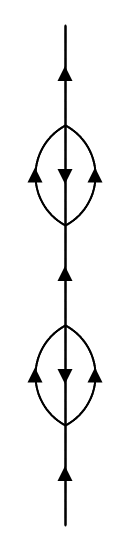
\includegraphics[height=6cm]{./figures/order4.png}
	\caption{one of fourth-order diagrams}
\end{figure}

It can be separated to two parts by a free Green function.
In a similar way, any diagram can be characterized as being either separable or non-separable with respect to cutting a single free fermion line. 
Thus, we can define the proper self-energy $\Sigma$ as summation over all non-separable diagrams.

Obviously, improper self-energy and proper self-energy are related by:

\begin{minipage}{0.12\textwidth}
	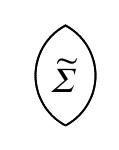
\includegraphics[height=2cm]{./figures/improper.png}
\end{minipage}
\begin{minipage}{0.02\textwidth}
	=
\end{minipage}
\begin{minipage}{0.12\textwidth}
	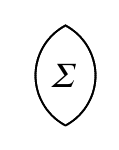
\includegraphics[height=2cm]{./figures/proper1.png}
\end{minipage}
\begin{minipage}{0.02\textwidth}
	+
\end{minipage}
\begin{minipage}{0.12\textwidth}
	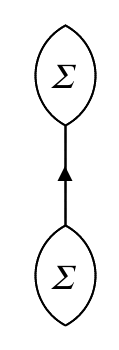
\includegraphics[height=4cm]{./figures/proper2.png}
\end{minipage}
\begin{minipage}{0.02\textwidth}
	+
\end{minipage}
\begin{minipage}{0.12\textwidth}
	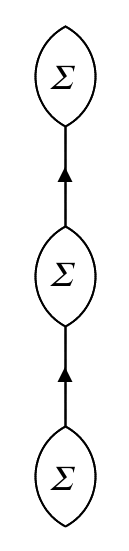
\includegraphics[height=6cm]{./figures/proper3.png}
\end{minipage}
\begin{minipage}{0.2\textwidth}
	+ \qquad \dots
\end{minipage}

or algebraicly by
\begin{equation}
	\tilde{\boldsymbol{\Sigma}}(\omega)=\boldsymbol{\Sigma}(\omega)+\boldsymbol{\Sigma}(\omega) \boldsymbol{G}^0(\omega) \tilde{\boldsymbol{\Sigma}}(\omega)
\end{equation}

Thus we can obtain the Dyson equation:
\begin{equation}
	\boldsymbol{G}(\omega)=\boldsymbol{G}^{0}(\omega)+\boldsymbol{G}^{0}(\omega) \boldsymbol{\Sigma}(\omega) \boldsymbol{G}(\omega)
\end{equation}
and thus
\begin{equation}
	\boldsymbol{\Sigma}(\omega)=\boldsymbol{G}^{0}(\omega)^{-1}-\boldsymbol{G}(\omega)^{-1}
\end{equation}

Since both the improper and proper self-energy are defined by summation of diagrams, it is obvious that they can also be expanded just like Green functions.
For example, the second order of proper self-energy is
\begin{equation} \label{selforder2}
	\Sigma_{p q}^{(2)}(\omega)=\sum_{a, b, k} \frac{V_{p k[a b]} V_{a b[q k]}}{\omega+\epsilon_{k}-\epsilon_{a}-\epsilon_{b}+i \eta}+\sum_{a, k, l} \frac{V_{p a[k l]} V_{k l[q a]}}{\omega+\epsilon_{a}-\epsilon_{k}-\epsilon_{l}-i \eta}
\end{equation}

THe self-energy can be written in a general form:
\begin{equation}
	\Sigma_{p q}(\omega)=\Sigma_{p q}(\infty)+M_{p q}(\omega)
\end{equation}
where $\Sigma_{p q}(\infty)$ and $M_{p q}(\omega)$ are refered to as dynamical part and static part, respectively.
It can be proved that $M_{pq}(\omega)$ can also be written in a spectral representation form:
\begin{equation}
	M_{p q}(\omega)=M_{p q}^{+}(\omega)+M_{p q}^{-}(\omega)=\sum_{\nu} \frac{m_{p}^{(\nu)} m_{q}^{(\nu) *}}{\omega-\omega_{\nu}+i \eta}+\sum_{\mu} \frac{m_{p}^{(\mu)} m_{q}^{(\mu) *}}{\omega-\omega_{\mu}-i \eta}
\end{equation}

The proof in given in reference \cite{Mpqproof1,Mpqproof2}.

If the infinite small $\eta$ is ignored, then 
\begin{equation}
	M_{p q}(\omega)=\sum_{\nu} \frac{m_{p}^{(\nu)} m_{q}^{(\nu) *}}{\omega-\omega_{\nu}}+\sum_{\mu} \frac{m_{p}^{(\mu)} m_{q}^{(\mu) *}}{\omega-\omega_{\mu}}
\end{equation}
and 
\begin{equation}
	G_{p q}(\omega)=\sum_{n} \frac{x_{p}^{n} x_{q}^{n *}}{\omega-e_{n}}
\end{equation}
where $n$ runs over both $N+1$ states and $N-1$ states.

Additionally,
\begin{equation}
	\begin{aligned}
		G_{p q}^{0}(\omega)&=\delta_{p q}\left(\frac{\overline{n}_{p}}{\omega-\varepsilon_{p}+i \eta}+\frac{n_{p}}{\omega-\varepsilon_{p}-i \eta}\right)
		\\
		&=\frac{\delta_{p q}}{\omega-\varepsilon_{p}}
	\end{aligned}
\end{equation}

In matrix representation,
\begin{equation}
	\boldsymbol{M}^{ \pm}(\omega)=\boldsymbol{m}^{ \pm \dagger}\left(\omega \mathbf{1}-\boldsymbol{\Omega}^{ \pm}\right)^{-1} \boldsymbol{m}^{ \pm}
\end{equation}
\begin{equation}
	\boldsymbol{G}(\omega)=\boldsymbol{x}(\omega \mathbf{1}-\boldsymbol{E})^{-1} \boldsymbol{x}^{\dagger}
\end{equation}
\begin{equation}
	\boldsymbol{G}^0(\omega)=(\omega \mathbf{1} - \boldsymbol{\epsilon})^{-1}
\end{equation}
and 
\begin{equation}
	\boldsymbol{x} \boldsymbol{x}^{\dagger}=1
\end{equation}

Since
\begin{equation}
	\begin{aligned} \boldsymbol{G}(\omega)^{-1} &=\omega\left[x\left(\mathbf{1}-\frac{\boldsymbol{E}}{\omega}\right)^{-1} \boldsymbol{x}^{\dagger}\right]^{-1} \\ &=\omega\left[\boldsymbol{x}\left(\mathbf{1}+\frac{\boldsymbol{E}}{\omega}+O\left(\omega^{-2}\right)\right) \boldsymbol{x}^{\dagger}\right]^{-1} \\ &=\omega\left[\mathbf{1}+\boldsymbol{x} \frac{\boldsymbol{E}}{\omega} \boldsymbol{x}^{\dagger}+O\left(\omega^{-2}\right)\right]^{-1}=\omega \mathbf{1}-x \boldsymbol{E} \boldsymbol{x}^{\dagger}+O\left(\frac{1}{\omega}\right) \end{aligned}
\end{equation}

We have 
\begin{equation}
	\begin{aligned}
		\boldsymbol{\Sigma}(\omega)&=\boldsymbol{G}^{0}(\omega)^{-1}-\boldsymbol{G}(\omega)^{-1}
		\\
		&=-\boldsymbol{\epsilon}+\boldsymbol{x} \boldsymbol{E} \boldsymbol{x}^{\dagger}+O\left(\frac{1}{\omega}\right)
	\end{aligned}
\end{equation}
and thus
\begin{equation}
	\boldsymbol{\Sigma}(\infty)=-\boldsymbol{\epsilon}+\boldsymbol{x} \boldsymbol{E} \boldsymbol{x}^{\dagger}
\end{equation}


As a result, the Dyson equation becomes:
\begin{equation}
	\boldsymbol{G}(\omega)=\left(\omega \mathbf{1}-\boldsymbol{\epsilon}-\boldsymbol{\Sigma}(\infty)-\boldsymbol{m}^{-\dagger}\left(\omega \mathbf{1}-\boldsymbol{\Omega}^{-}\right)^{-1} \boldsymbol{m}^{-}-\boldsymbol{m}^{+^{\dagger}}\left(\omega \mathbf{1}-\boldsymbol{\Omega}^{+}\right)^{-1} \boldsymbol{m}^{+}\right)^{-1}
\end{equation}

It can be proved that if we introduce Dyson secular matrix
\begin{equation} \label{matrixA}
	\boldsymbol{A}=\left( \begin{array}{ccc}{\boldsymbol{\epsilon}+\boldsymbol{\Sigma}(\infty)} & {\boldsymbol{m}^{-\dagger}} & {\boldsymbol{m}^{+\dagger}} \\ {\boldsymbol{m}^{-}} & {\boldsymbol{\Omega}^{-}} & {\mathbf{0}} \\ {\boldsymbol{m}^{+}} & {\mathbf{0}} & {\boldsymbol{\Omega}^{+}}\end{array}\right)
\end{equation}
then
\begin{equation}
	\boldsymbol{G}(\omega)=\left.(\omega \mathbf{1}-\boldsymbol{A})^{-1}\right|_{11}
\end{equation}
where the $11$ subscript means taking the upper left diagonal block.

Thus the energies interested, which are poles of $G$, are also poles of Dyson secular matrix $A$.

from Eq \ref{selforder2}, we can also determine the leading terms of $m$ and $\Omega$.
Since 
\begin{equation}
	\begin{aligned} 
	M_{p q}^{(2)+}(\omega) &=\sum_{a<b, k} \frac{V_{p k[a b]} V_{a b[q k]}}{\omega+\epsilon_{k}-\epsilon_{a}-\epsilon_{b}+i \eta}
	\\ 
	M_{p q}^{(2)-}(\omega) &=\sum_{a, k<l} \frac{V_{p a[k l]} V_{k l[q a]}}{\omega+\epsilon_{a}-\epsilon_{k}-\epsilon_{l}-\epsilon_{l}-i \eta}
	\end{aligned}
\end{equation}
we have
\begin{equation}
	\begin{aligned} 
	\Omega_{a k l, a k l}^{-} &=-\epsilon_{a}+\epsilon_{k}+\epsilon_{l}
	\\ 
	\Omega_{a b k, a b k}^{+} &=-\epsilon_{k}+\epsilon_{a}+\epsilon_{b} 
	\end{aligned}
\end{equation}
and
\begin{equation} 
	m_{a k l, q}^{-} =V_{q a[k l]}, \quad m_{a b k, q}^{+}=V_{a b[q k]}
\end{equation}

They are leading terms since the leading order of $M$ is second order.
This is because
\begin{equation}
	\begin{aligned}
		\boldsymbol{\Sigma}(\omega)&=\boldsymbol{G}^{0}(\omega)^{-1}-\boldsymbol{G}(\omega)^{-1}
		\\
		&=\boldsymbol{G}^{0}(\omega)^{-1}-(\boldsymbol{G}^0(\omega)+O(2))^{-1}
		\\
		&=O(2)
	\end{aligned}
\end{equation}

As is mentioned previously, a finite perturbation expansion of the electron propagator does not reproduce its correct analytical form.
However, we are still useing finite perturbation expansion, i.e. determine each order of $m$, $\Omega$ and then calcuate the eigenvalues of Dyson secular matrix in Eq \ref{matrixA}.

We will then begin introducing ADC to sum partially to infitity.
We will consider $M^{+}$ in the following since it is analogous for $M^{-}$.

In ADC, equation 
\begin{equation}
	M_{p q}(\omega)=\boldsymbol{m}_{p}^{\dagger}(\omega \mathbf{1}-\boldsymbol{\Omega})^{-1} \boldsymbol{m}_{q}
\end{equation}
is replaced by ADC form:
\begin{equation}
	M_{p q}(\omega)=\boldsymbol{U}_{p}^{\dagger}(\omega \mathbf{1}-\boldsymbol{K}-\boldsymbol{C})^{-1} \boldsymbol{U}_{q}
\end{equation}
where
$\boldsymbol{K}+\boldsymbol{C}$ is refered to as ADC secular matrix.

Although $\boldsymbol{K}$, $\boldsymbol{C}$, and $\boldsymbol{U}$ are not specified yet,
we may suppose that the following perturbation expansions apply:
\begin{equation} \label{cuexpansion}
	\begin{aligned} 
		\boldsymbol{C} &=\boldsymbol{C}^{(1)}+\boldsymbol{C}^{(2)}+\cdots 
		\\ 
		\boldsymbol{U_{p}} &=\boldsymbol{U_{p}}^{(1)}+\boldsymbol{U_{p}}^{(2)}+\cdots
	\end{aligned}
\end{equation}

Here $\boldsymbol{K}$ is actually the zeroth order of $\boldsymbol{C}$.
Thus
\begin{equation}
	\begin{array}{l}{K_{j a b, j a b}=-\epsilon_{j}+\epsilon_{a}+\epsilon_{b}} \\ {K_{i j a b c, i j a b c}=-\epsilon_{i}-\epsilon_{j}+\epsilon_{a}+\epsilon_{b}+\epsilon_{c}} \\ {\qquad \vdots}\end{array}
\end{equation}
where $i, j, k \dots$ label occupied orbitals while $a, b, c \dots$ label virtual orbitals.

Although we still expand $\boldsymbol{K}$ and $\boldsymbol{C}$ to finite order, the expansion of $M$ is already partially to infinite orders:
\begin{equation} \label{adcexpansion}
	\begin{aligned} M_{p q}(\omega) &=\boldsymbol{U}_{p}^{\dagger}(\omega \mathbf{1}-\boldsymbol{K}-\boldsymbol{C})^{-1} \boldsymbol{U}_{q} \\ &=\boldsymbol{U}_{p}^{\dagger}(\omega \mathbf{1}-\boldsymbol{K})^{-1} \sum_{n=0}^{\infty}\left\{\boldsymbol{C}(\omega \mathbf{1}-\boldsymbol{K})^{-1}\right\}^{n} \boldsymbol{U}_{q} \end{aligned}
\end{equation}

Now, we can formulate the ADC procedure as follows:

Compare the formal perturbation expansion of the ADC form Eq \ref{adcexpansion} to the original diagrammatic perturbation expansion for the self-energy part $M^{+}_{pq}(\omega)$ through a given order $n$ of perturbation theory.
Beginning at second order and proceeding to higher order, this comparison allows one to determine successively the terms in the expansions Eq \ref{cuexpansion} of $\boldsymbol{C}$ and $\boldsymbol{U}_p$ , respectively.

Through second order of $M$, we can determine $\boldsymbol{C}$ and $\boldsymbol{U}_p$ as
\begin{equation}
	U_{j a b, q}^{(1)}=V_{a b[q j]}
\end{equation}
\begin{equation}
	C_{j a b, j^{\prime} a^{\prime} b^{\prime}}=0
\end{equation}

Through third order of $M$, we can determine $\boldsymbol{C}$ and $\boldsymbol{U}_p$ as
\begin{equation}
	\begin{aligned} 
		U_{j a b, q}^{(2)}&= \frac{1}{2} \sum_{k l} \frac{V_{a b[k l]} V_{k l[q j]}}{\epsilon_{k}+\epsilon_{l}-\epsilon_{a}-\epsilon_{b}} +\left(\sum_{c k} \frac{V_{a c[k j]} V_{k b[q c]}}{\epsilon_{a}+\epsilon_{c}-\epsilon_{j}-\epsilon_{k}}\right)-(a \leftrightarrow b)
		\\
		C_{j a b, j^{\prime} a^{\prime} b^{\prime}}^{(1)}&=\delta_{j j^{\prime}} V_{a b\left[a^{\prime} b^{\prime}\right]}-\left(\delta_{a a^{\prime}} V_{j^{\prime} b\left[j b^{\prime}\right]}+\delta_{b b^{\prime}} V_{j^{\prime} a\left[j a^{\prime}\right]}\right)+(a^{\prime} \leftrightarrow b^{\prime})
	 \end{aligned}
\end{equation}

Instead of Dyson secular matrix, we have a new Dyson-ADC secular matrix:
\begin{equation}
	\boldsymbol{B}=\left( \begin{array}{ccc}{\epsilon+\mathbf{\Sigma}(\infty)} & {\boldsymbol{U}^{-\dagger}} & {\boldsymbol{U}^{+\dagger}} \\ {\boldsymbol{U}^{-}} & {\boldsymbol{K}^{-}+\boldsymbol{C}^{-}} & {\mathbf{0}} \\ {\boldsymbol{U}^{+}} & {\boldsymbol{0}} & {\boldsymbol{K}^{+}+\boldsymbol{C}^{+}}\end{array}\right)
\end{equation}
and
\begin{equation}
	\boldsymbol{G}(\omega)=\left.(\omega \mathbf{1}-\boldsymbol{B})^{-1}\right|_{11}
\end{equation}

The struture of Dyson-ADC(3) matrix is:
\begin{table}
	\centering
	\begin{tabular}{c|c|c|c|}
		   &   1h/1p  &   2h-1p &  2p-1
		\\
		\hline
		1h/1p  &  $\boldsymbol{\epsilon}+\boldsymbol{\Sigma}(\infty)$ & $U^{-(1,2)\dagger}$ & $ U^{+(1,2)\dagger} $
		\\
		\hline
		2h-1p &  $U^{-(1,2)\dagger}$ & $K^{-}+C^{-(1)}$ & 0
		\\
		\hline
		2p-1h &  $U^{+(1,2)\dagger}$ & 0 & $K^{+}+C^{+(1)}$
		\\
		\hline
	\end{tabular}
\end{table}

The summation to infitity ensures that Dyson-ADC is a size consistent method, which is an important advantage over CI.
Another advatange is that configuration space of Dyson-ADC is smaller than CI.
For example, The consis- tent treatment of 1h main states through second (and third order) requires the CI expansions to extend through the 3h-2p configurations.
By contrast, the ADC(2) (and ADC(3)) configuration spaces are restricted to the 2h-1p configurations of $N−1$ particles, but also comprise the 2h-1p configurations of $N+1$ particles.

\subsection{Non-dyson approach}
The advantage of Dyson approach is the decrease the number of feyman diagrams one need to calculate by property of Dyson equation.
However, the problem is that $N+1$ part and $N-1$ part are coupled, thus one has to diagonalize the full B matrix.
Moreover, people usually care about the first few ionized or electron affinitized states, which lie in the middle of the energy spectrum.
Algorithmically, it is difficult to determine eigenvalues in the middle part of an energy spectrum.
Thus, we introduce Non-dyson approach, which solve this problem and make sure that all states interested are in the edge of energy spectrum
Since Non-dyson ADC treat $N+1$ part and $N-1$ part separately, we will focus on $N-1$ part, and $N+1$ part is analogous.

Related to $N-1$ part, Green funtion $G^{-}$ can be written as
\begin{equation}
	\boldsymbol{G}^{-}(\omega)=\boldsymbol{x}(\omega \mathbf{1}-\boldsymbol{\Omega})^{-1} \boldsymbol{x}^{\dagger}
\end{equation}
where $\Omega$ are negative ionization energies that we do care about.

By transposing, we obtain
\begin{equation}
	\tilde{\boldsymbol{G}}(\omega)=\boldsymbol{G}^{-}(\omega)^{t}=\tilde{\boldsymbol{x}}^{\dagger}(\omega \mathbf{1}-\boldsymbol{\Omega})^{-1} \tilde{\boldsymbol{x}}
\end{equation}

Then we introduce ADC representation just like Dyson approach:
\begin{equation}
	\tilde{\boldsymbol{G}}(\omega)=\boldsymbol{f}^{\dagger}(\omega-\boldsymbol{K}-\boldsymbol{C})^{-1} \boldsymbol{f}
\end{equation}

Just like Dyson approach, we still expand $\boldsymbol{C}$ and $\boldsymbol{g}$ to series:
\begin{equation}
	\begin{aligned} \boldsymbol{K}+\boldsymbol{C} &=\boldsymbol{K}+\boldsymbol{C}^{(1)}+\boldsymbol{C}^{(2)}+\boldsymbol{C}^{(3)}+\ldots \\ \boldsymbol{f} &=\boldsymbol{f}^{(0)}+\boldsymbol{f}^{(1)}+\boldsymbol{f}^{(2)}+\ldots \end{aligned}
\end{equation}
where the expression for $\boldsymbol{K}$ is:
\begin{equation}
	\begin{aligned} K_{k k} &=\epsilon_{k} \\ K_{a k l, a k l} &=\epsilon_{k}+\epsilon_{l}-\epsilon_{a} \\ & \vdots \end{aligned}
\end{equation}

Just like Dyson approach, we can also see that the expansion of $M$ is partially to infinite orders:
\begin{equation}
	\tilde{\boldsymbol{G}}(\omega)=\boldsymbol{f}^{\dagger}(\omega-\boldsymbol{K}-\boldsymbol{C})^{-1} \boldsymbol{f}=\boldsymbol{f}^{\dagger}(\omega-\boldsymbol{K})^{-1} \sum_{\nu=0}^{\infty}\left(\frac{\boldsymbol{C}}{\omega-\boldsymbol{K}}\right)^{\nu} f
\end{equation}

The procedure of Non-dyson ADC is the same with Dyson-ADC.
By this procedure, we obtain the first few orders of $\boldsymbol{C}$ and $\boldsymbol{f}$ for Non-dyson ADC(2):

\begin{equation}
	\begin{aligned}
		f_{p q}^{(0)}&=\delta_{p q} n_{p}
		\\
		f_{\mu}^{(0)}&=0, \text { for } \mu>1
		\\
		f_{1}^{(1)}&=\mathbf{0} \text { for } \mu>2
		\\
		f_{a k l, q}^{(1)}&=\frac{V_{q a[k] ]}}{\epsilon_{q}+\epsilon_{a}-\epsilon_{k}-\epsilon_{l}} \overline{n}_{q}
		\\
		f_{p q}^{(2)}&=\frac{1}{4} \sum_{a, b, j} v_{a b p j} v_{q j a b} n_{q}
		\\
		C_{11}^{(1)}&=0
		\\
		C_{1 \mu}^{(1)}&=0 \text { for } \mu>2
		\\
		C_{p, a k l}^{(1)}&=-V_{k l[p a]} n_{p}
		\\
		C_{p q}^{(2)}&=\frac{1}{2} \sum_{a, b, j} v_{a b p j} v_{q j a b}\left(\epsilon_{a}+\epsilon_{b}-\epsilon_{j}-\frac{1}{2} \epsilon_{p}-\frac{1}{2} \epsilon_{q}\right), n_{p}=n_{q}=1
	\end{aligned}
\end{equation}

We can also use \ref{greenenergy} to calculate ground state energy by Non-dyson ADC.
\begin{equation}
	\begin{aligned}
		\boldsymbol{\rho}&=\frac{1}{2 \pi i} \oint \boldsymbol{G}^{-}(\omega) \mathrm{d} \omega
		\\
		&=\frac{1}{2 \pi i} \oint f^{\dagger}(\omega-K-C)^{-1} f \mathrm{d} \omega=f^{\dagger} f
	\end{aligned}
\end{equation}

Thus
\begin{equation}
	E_{0}=\frac{1}{2} \operatorname{Tr}\left(f^{\dagger}(\boldsymbol{K}+\boldsymbol{C}) \boldsymbol{f}+\boldsymbol{T}^{t} \boldsymbol{f}^{\dagger} \boldsymbol{f}\right)
\end{equation}

The complexity of Non-dyson ADC(2) is $m^4$ while ADC(3) is $m^5$, where $m$ is the number of one particle basis.

It can be proved that Non-dyson ADC is also size consistent.
The reason is that the direct ADC secular matrix can be identified as the representation of the (subtracted) Hamiltonian with respect to a specific set of intermediate states, which will be presented in the next section.

